% Created 2019-11-04 月 20:22
% Intended LaTeX compiler: pdflatex
\documentclass[dvipdfmx,11pt]{jarticle}
\usepackage[utf8]{inputenc}
\usepackage[T1]{fontenc}
\usepackage{graphicx}
\usepackage{grffile}
\usepackage{longtable}
\usepackage{wrapfig}
\usepackage{rotating}
\usepackage[normalem]{ulem}
\usepackage{amsmath}
\usepackage{textcomp}
\usepackage{amssymb}
\usepackage{capt-of}
\usepackage{hyperref}
\setlength{\textwidth}{18cm}
\setlength{\oddsidemargin}{-1cm}
\setlength{\evensidemargin}{-1cm}
\setlength{\topmargin}{-2cm}
\setlength{\textheight}{26cm}
\setcounter{secnumdepth}{6}
\author{suzuki@iwate-u.ac.jp 鈴木正幸,岩手大学・非常勤講師}
\date{2019.11.05}
\title{数理情報科学特論 コンピュータと数式処理\\
https://github.com/masayuki054/comp\_and\_cal
}
\begin{document}

\maketitle

\section{デジタル技術と協調しよう}
\label{sec:orgbc2b862}

コンピュータとインターネットと上手に付き合って,
知り,考え,記憶し,検索し,思い出せるようにしましょう。

\begin{itemize}
\item \href{./org/digital\_tools.org}{思考とメモと文書のためのデジタル・ツール}
\begin{itemize}
\item 知識は構造
\item アウトライナー
\item マインドマップ
\item 文芸的プログラミング
\end{itemize}

\item \href{./org/web.org}{Web進化論}
\begin{itemize}
\item 集合知
\item 知識の構造化
\end{itemize}

\item \href{./org/comp\_thinking.org}{計算論的思考}
\begin{itemize}
\item computer科学者のように考え,問題に取り組み,システムをデザイン
しよう
\end{itemize}

\item \href{./org/math-soft.org}{数学ソフトウェア}
\begin{itemize}
\item フリーソフトウェアを利用しよう
\item 数式処理システムと計算機代数アルゴリズム
\end{itemize}
\end{itemize}

\section{規則と簡約化と検索のための計算機代数}
\label{sec:orga367cf4}

数学と検索と簡約のつながりについて,考えます。人は理論を考え,コン
ピュータに検索してもらいましょう。

多くの変数の高い次数の方程式の解法を,
線形代数の概念に翻訳し,
線形空間の概念と計算に帰着します。見通しと効率が良くなります。

\begin{itemize}
\item \href{./org/groebner.org}{グレブナー基底} 計算機代数アルゴリズムの紹介
\end{itemize}

\begin{figure}[htbp]
\centering
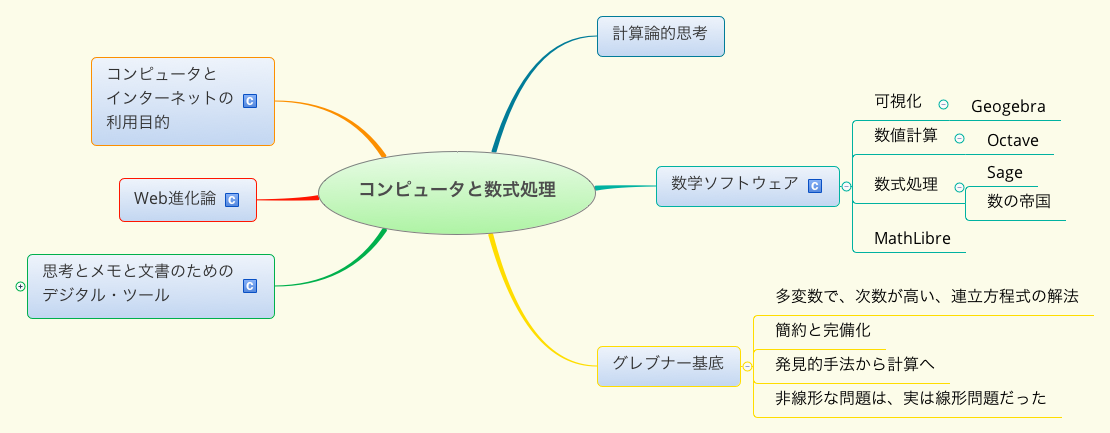
\includegraphics[width=14cm]{./map-images/01-computer_and_cal.png}
\caption{概要}
\end{figure}

\begin{figure}[htbp]
\centering
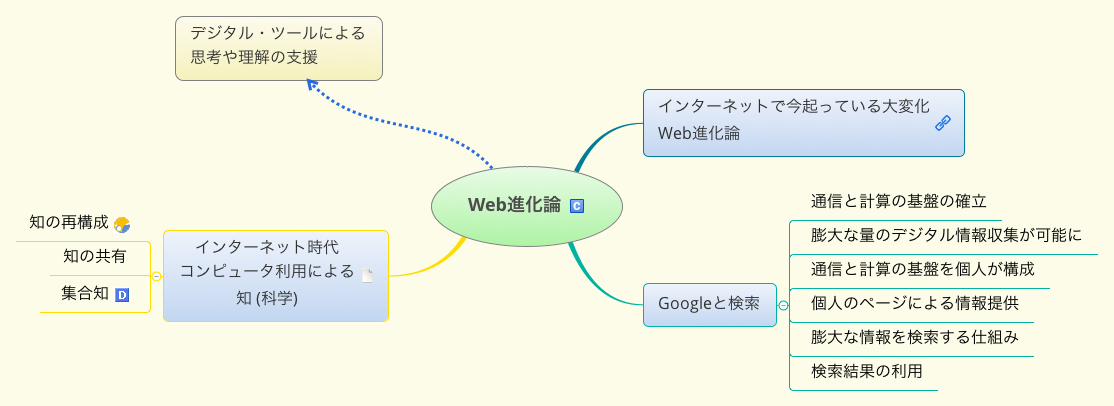
\includegraphics[width=14cm]{./map-images/04-Web_revolution.png}
\caption{インターネットが起している変革}
\end{figure}

\begin{figure}[htbp]
\centering
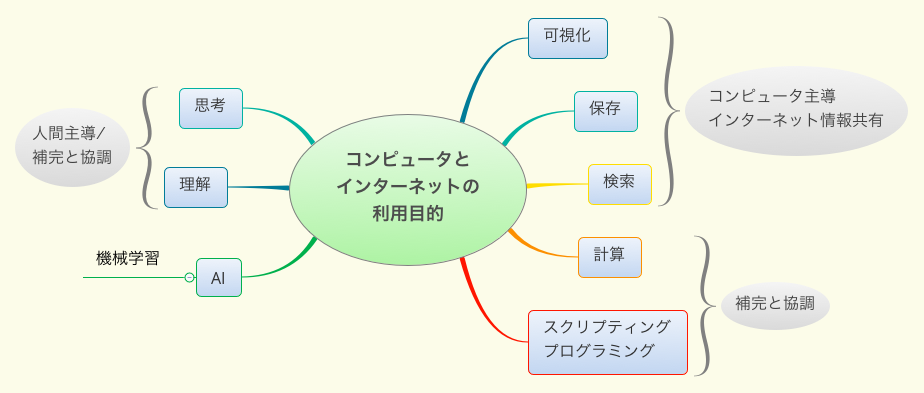
\includegraphics[width=14cm]{./map-images/03-how_to_use_computer_and_internet.png}
\caption{人とコンピュータとインターネット}
\end{figure}

\begin{figure}[htbp]
\centering
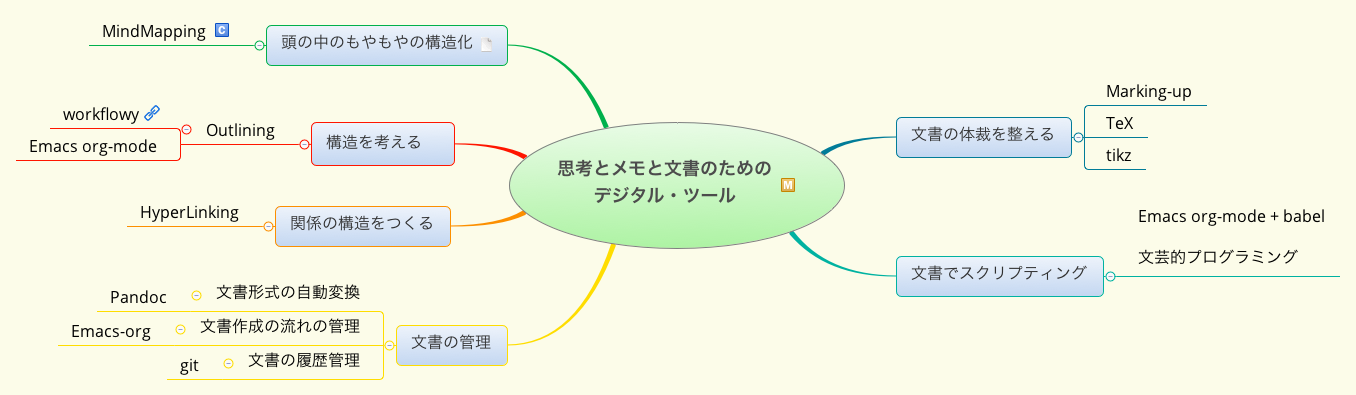
\includegraphics[width=14cm]{./map-images/05-digital_tools_for_thinking.png}
\caption{思考とメモと文書のためのデジタル・ツール}
\end{figure}
\end{document}
